\section{Gamma-Type Distributions}
\subsection{Gamma-Type Distributions}

The gamma family is a generalization of several important distributions (exponential, chi-square, Erlang) and frequently arises when modeling \emph{waiting times}.

\subsubsection{Gamma Function}

\begin{definicion}[Gamma Function]
The \emph{gamma function} $\Gamma: (0,\infty) \to \mathbb{R}$ is defined as
\begin{align}
 \label{eq:2.8.6}
 \Gamma(\alpha) = \int_0^\infty t^{\alpha-1} e^{-t}\,dt.
\end{align}
\end{definicion}

{Properties of the gamma function}
\begin{itemize}
 \item $\Gamma(1) = 1$.
 \item $\Gamma(\alpha + 1) = \alpha\,\Gamma(\alpha)$ for all $\alpha > 0$.
 \item In particular, for $\alpha \in \mathbb{N}$ we have $\Gamma(n) = (n-1)!$.
 \item $\Gamma(1/2) = \sqrt{\pi}$.
\end{itemize}

\subsubsection{Gamma Distribution}

\begin{definicion}[Gamma Distribution]
A continuous random variable $X$ has a \emph{gamma distribution} with shape parameter $\alpha > 0$ and scale parameter $\beta > 0$ if its density function is
\begin{align}
 \label{eq:2.8.7}
 f(x) =
 \begin{cases}
  \dfrac{1}{\Gamma(\alpha)\,\beta^\alpha}\,x^{\alpha-1}\,e^{-x/\beta},
  & x > 0, \\
  0, & \text{otherwise.}
 \end{cases}
\end{align}
We write $X \sim \text{Gamma}(\alpha, \beta)$.
\end{definicion}

{Properties of the gamma distribution} If $X \sim \text{Gamma}(\alpha, \beta)$, then
\begin{align}
 \mu_X &= \alpha\beta, \\
 \s_X^2 &= \alpha\beta^2.
\end{align}

\subsection{Exponential Distribution}

The exponential distribution models the waiting time until the occurrence of an event
when events occur continuously and independently at a constant rate (for example, the
time between calls arriving at a call center, or the lifetime of an electronic component
until its first failure).

\begin{definicion}[Exponential Distribution]
A continuous random variable $X$ has an \emph{exponential distribution} with rate
parameter $\lambda > 0$ if its density function is
\begin{align}
 \label{eq:2.8.8}
 f(x) =
 \begin{cases}
  \lambda\,e^{-\lambda x}, & x \geq 0, \\
  0, & \text{otherwise.}
 \end{cases}
\end{align}
We write $X \sim \text{Exp}(\lambda)$.
\end{definicion}

{Properties of the exponential distribution} If $X \sim \text{Exp}(\lambda)$, then
\begin{align}
 \mu_X &= \frac{1}{\lambda}, \\
 \s_X^2 &= \frac{1}{\lambda^2}.
\end{align}

\begin{observacion}[Memoryless Property]
The exponential distribution satisfies the \emph{memoryless property}: for $s, t \geq 0$,
\begin{align}
 P(X > s + t \mid X > s) = P(X > t).
\end{align}
It is the only continuous distribution (along with the geometric distribution in the discrete case) possessing this property.
\end{observacion}

The exponential distribution with parameter $\lambda$ corresponds exactly to the special
case $\text{Gamma}(1, \beta)$ of the gamma family, with $\lambda = 1/\beta$. This
identification explains, among other things, why the sum of $n$ independent
exponentials with the same rate follows a Gamma distribution, as shown below.

\subsubsection{Special Case: Chi-Square Distribution}

The chi-square distribution with $\nu$ degrees of freedom, denoted $\chi^2_\nu$, is a special case of the gamma distribution with parameters $\alpha = \nu/2$ and $\beta = 2$:
\begin{align}
 \label{eq:2.8.9}
 X \sim \chi^2_\nu \iff X \sim \text{Gamma}\!\left(\frac{\nu}{2}, 2\right).
\end{align}
Its density function is
\begin{align}
 f(x) = \frac{1}{2^{\nu/2}\,\Gamma(\nu/2)}\,x^{\nu/2-1}\,e^{-x/2}, \qquad x > 0.
\end{align}

This distribution is studied in detail in Section \ref{sec:3.9} of the inference chapter; its connection with the gamma family allows generalizing several of its properties.

\subsubsection{Sum of Independent Gamma Variables}

\begin{teorema}[Gamma Additive Property]
If $X_1, X_2, \dots, X_n$ are independent random variables with $X_i \sim \text{Gamma}(\alpha_i, \beta)$ (with the same scale $\beta$), then
\begin{align}
 \label{eq:2.8.10}
 Y = X_1 + X_2 + \cdots + X_n \sim \text{Gamma}\!\left(\sum_{i=1}^n \alpha_i,\, \beta\right).
\end{align}
\end{teorema}

\begin{ejemplo}
 \label{exmp:2.8.3}
Calls arrive at a call center according to a Poisson process with rate $\lambda = 3$ calls per minute. What is the distribution of the time until the third call? What is the probability that this time is greater than $1.5$ minutes?
\end{ejemplo}

\begin{solucion}
The time between consecutive calls is exponential with parameter $\lambda = 3$, i.e., $T_i \sim \text{Exp}(3)$ with mean $1/3$ minutes.

By the additive property of the gamma distribution, the time until the third call is
\begin{align}
 T = T_1 + T_2 + T_3 \sim \text{Gamma}(3, 1/3).
\end{align}
Equivalently, $T \sim \text{Erlang}(3, 3)$ with rate parameter $3$.

The probability that $T > 1.5$ is
\begin{align}
 P(T > 1.5) = 1 - F_{\text{Gamma}}(1.5; 3, 1/3) = e^{-3 \cdot 1.5}\left(1 + 3\cdot 1.5 + \frac{(3\cdot 1.5)^2}{2}\right).
\end{align}

Numerically: $3 \cdot 1.5 = 4.5$, so
\begin{align}
 P(T > 1.5) = e^{-4.5}\left(1 + 4.5 + \frac{20.25}{2}\right) = e^{-4.5}(15.625) \approx 0.174.
\end{align}
\end{solucion}

\lstinputlisting[language=Python]{../code/distribuciones-continuas-avanzadas/distGamma.py}

\begin{figure}
 \centering
 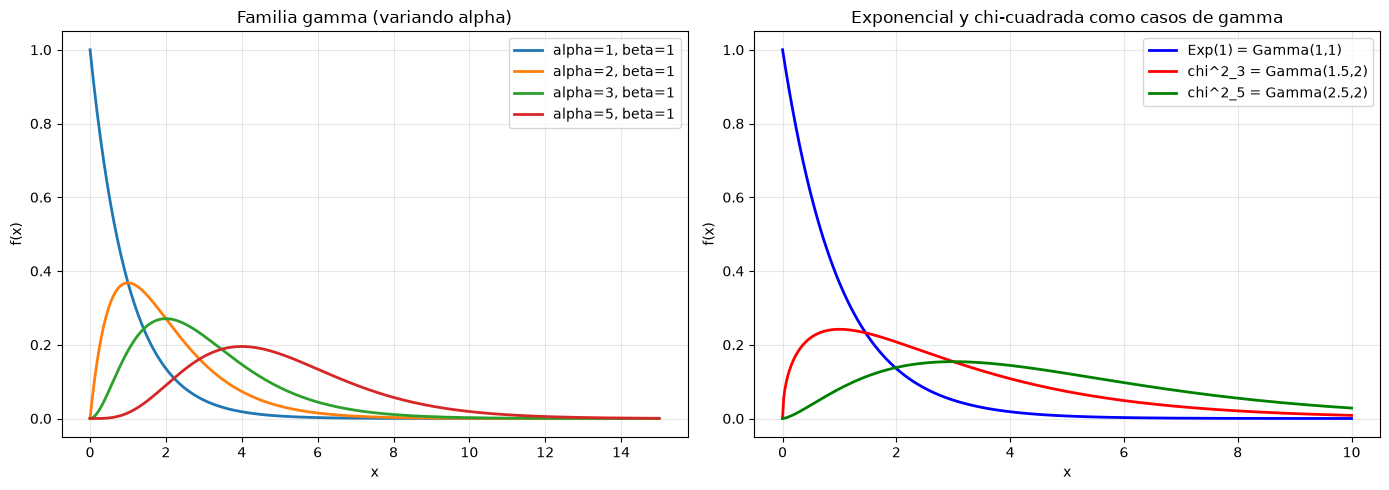
\includegraphics[height=7cm,keepaspectratio=true]{./pe/distGamma.png}
 % distGamma.png: 0x0 pixel, 300dpi, 0.00x0.00 cm, bb=
 \caption{Gamma family and its special cases (exponential and chi-square).}
 \label{fig:2.8.3}
\end{figure}

\subsection{Beta Distribution}

The beta distribution models continuous random variables restricted to the interval
$[0,1]$, making it ideal for representing proportions, unknown probabilities, or
fractions. Together with the gamma function, the beta function is a classical calculus
tool that connects both distribution families.

\begin{definicion}[Beta Function]
The \emph{beta function} $B: (0,\infty)\times(0,\infty) \to \mathbb{R}$ is defined as
\begin{align}
 \label{eq:2.8.16}
 B(\alpha,\beta) = \int_0^1 t^{\alpha-1}(1-t)^{\beta-1}\,dt
 = \frac{\Gamma(\alpha)\,\Gamma(\beta)}{\Gamma(\alpha+\beta)}.
\end{align}
\end{definicion}

\begin{definicion}[Beta Distribution]
A continuous random variable $X$ has a \emph{beta distribution} with shape parameters
$\alpha > 0$ and $\beta > 0$ if its density function is
\begin{align}
 \label{eq:2.8.17}
 f(x) =
 \begin{cases}
  \dfrac{1}{B(\alpha,\beta)}\,x^{\alpha-1}(1-x)^{\beta-1}, & 0 < x < 1, \\
  0, & \text{otherwise.}
 \end{cases}
\end{align}
We write $X \sim \text{Beta}(\alpha,\beta)$.
\end{definicion}

{Properties of the beta distribution} If $X \sim \text{Beta}(\alpha,\beta)$, then
\begin{align}
 \mu_X &= \frac{\alpha}{\alpha+\beta}, \\
 \s_X^2 &= \frac{\alpha\beta}{(\alpha+\beta)^2(\alpha+\beta+1)}.
\end{align}

\begin{observacion}
When $\alpha=\beta=1$, the beta distribution reduces to the $U(0,1)$ distribution.
Moreover, because it is bounded on $[0,1]$, the beta distribution is the classical
\emph{conjugate prior} for the parameter $p$ of a Bernoulli or Binomial distribution in
Bayesian inference: if the prior belief about $p$ is $\text{Beta}(\alpha,\beta)$ and $k$
successes are observed in $n$ trials, the updated (posterior) belief is
$\text{Beta}(\alpha+k,\, \beta+n-k)$.
\end{observacion}

\begin{ejemplo}
 \label{exmp:2.8.7}
A quality control report indicates that the proportion $X$ of defective items in a batch
follows a $\text{Beta}(2,8)$ distribution. What is the expected proportion of defective
items? What is the variance?
\end{ejemplo}

\begin{solucion}
Since $X \sim \text{Beta}(2,8)$,
\begin{align}
 E(X) = \frac{\alpha}{\alpha+\beta} = \frac{2}{10} = 0.2,
\end{align}
that is, we expect $20\%$ of the items to be defective.

The variance is
\begin{align}
 \text{Var}(X) = \frac{\alpha\beta}{(\alpha+\beta)^2(\alpha+\beta+1)}
 = \frac{2\cdot 8}{10^2 \cdot 11} = \frac{16}{1100} \approx 0.0145.
\end{align}
\end{solucion}

\subsection{Weibull Distribution}

The Weibull distribution generalizes the exponential distribution by allowing the
\emph{failure rate} (or \emph{hazard function}) to vary over time, making it widely used
in reliability analysis and lifetime studies of components.

\begin{definicion}[Weibull Distribution]
A continuous random variable $T \geq 0$ has a \emph{Weibull distribution} with shape
parameter $\beta > 0$ and scale parameter $\eta > 0$ if its density function is
\begin{align}
 \label{eq:2.8.18}
 f(t) =
 \begin{cases}
  \dfrac{\beta}{\eta}\left(\dfrac{t}{\eta}\right)^{\beta-1}
  \exp\!\left[-\left(\dfrac{t}{\eta}\right)^{\beta}\right], & t \geq 0, \\
  0, & \text{otherwise.}
 \end{cases}
\end{align}
We write $T \sim \text{Weibull}(\beta,\eta)$.
\end{definicion}

Its cumulative distribution function has a closed form:
\begin{align}
 \label{eq:2.8.19}
 F(t) = 1 - \exp\!\left[-\left(\dfrac{t}{\eta}\right)^{\beta}\right], \qquad t \geq 0.
\end{align}

{Hazard function (failure rate)} For a lifetime variable $T$ with density $f$ and
reliability $R(t) = 1 - F(t)$, the \emph{hazard function} is defined as $h(t) =
f(t)/R(t)$. For $T \sim \text{Weibull}(\beta,\eta)$,
\begin{align}
 \label{eq:2.8.20}
 h(t) = \frac{\beta}{\eta}\left(\frac{t}{\eta}\right)^{\beta-1}.
\end{align}

\begin{observacion}
The shape parameter $\beta$ determines the behavior of the failure rate:
\begin{itemize}
 \item If $\beta = 1$, $h(t)$ is constant and $T \sim \text{Exp}(1/\eta)$ (random
 failure, no aging).
 \item If $\beta < 1$, $h(t)$ is decreasing (infant mortality: early failures due to
 manufacturing defects).
 \item If $\beta > 1$, $h(t)$ is increasing (wear-out: the failure probability
 increases with the component's age).
\end{itemize}
\end{observacion}

{Properties of the Weibull distribution} If $T \sim \text{Weibull}(\beta,\eta)$, then
\begin{align}
 \mu_T &= \eta\,\Gamma\!\left(1 + \frac{1}{\beta}\right), \\
 \s_T^2 &= \eta^2\left[\Gamma\!\left(1 + \frac{2}{\beta}\right)
 - \Gamma\!\left(1 + \frac{1}{\beta}\right)^2\right].
\end{align}

\begin{ejemplo}
 \label{exmp:2.8.8}
The lifetime $T$ (in thousands of hours) of an electronic component follows a
$\text{Weibull}(\beta=2, \eta=5)$ distribution. What is the probability that the
component fails before $3000$ hours? Is the failure rate increasing or decreasing?
\end{ejemplo}

\begin{solucion}
Since $T \sim \text{Weibull}(2,5)$ (with $T$ in thousands of hours), we want $P(T < 3) =
F(3)$:
\begin{align}
 F(3) = 1 - \exp\!\left[-\left(\frac{3}{5}\right)^2\right]
 = 1 - e^{-0.36} \approx 1 - 0.6977 = 0.3023.
\end{align}
Therefore, there is approximately a $30.23\%$ probability of failure before $3000$
hours.

Since $\beta = 2 > 1$, the failure rate $h(t) = \frac{2}{5}\left(\frac{t}{5}\right)$ is
\emph{increasing}: the component exhibits a wear-out pattern, with higher failure risk
as it ages.
\end{solucion}

